% \documentclass[aspectratio=169, 11pt]{beamer}
\documentclass[aspectratio=169, 11pt, handout]{beamer}

% ── Theme ──
\usetheme{Madrid}
\usecolortheme{default}
\setbeamertemplate{navigation symbols}{}
\setbeamertemplate{footline}{%
  \leavevmode\hbox{%
    \begin{beamercolorbox}[wd=.333333\paperwidth,ht=2.5ex,dp=1ex,center]{author in head/foot}%
      \usebeamerfont{author in head/foot}\insertshortauthor
    \end{beamercolorbox}%
    \begin{beamercolorbox}[wd=.333333\paperwidth,ht=2.5ex,dp=1ex,center]{title in head/foot}%
      \usebeamerfont{title in head/foot}\insertshorttitle
    \end{beamercolorbox}%
    \begin{beamercolorbox}[wd=.333333\paperwidth,ht=2.5ex,dp=1ex,right]{date in head/foot}%
      \usebeamerfont{date in head/foot}\insertframenumber{} / \inserttotalframenumber\hspace*{2ex}
    \end{beamercolorbox}}}

% ── Packages ──
\usepackage{amsmath,amssymb}
\usepackage{booktabs}
\usepackage{xcolor}
\usepackage{colortbl}
\usepackage{graphicx}
\usepackage{tikz}
\usetikzlibrary{arrows.meta, positioning, calc}

% ── Colors ──
\definecolor{sbgreen}{HTML}{00704A}  % course accent
\definecolor{warnred}{HTML}{CC0000}
\definecolor{noteblue}{HTML}{2060A0}

% ── Commands ──
\newcommand{\E}{\mathbb{E}}
\newcommand{\Var}{\mathrm{Var}}
\newcommand{\Cov}{\mathrm{Cov}}
\newcommand{\SE}{\mathrm{SE}}
\newcommand{\Prob}{\mathrm{Pr}}
\newcommand{\indep}{\perp\!\!\!\perp}

\usepackage{soul}
\newcommand{\NUM}[2]{\sethlcolor{yellow}\hl{#1\,\textsuperscript{?}}\marginpar{\tiny #2}}
% Beamer frames are typeset inside boxes, where \marginpar raises "Not in outer par mode"
% and \marginparwidth is 4pt. Same marker; the provenance note goes to the frame footnote.
\renewcommand{\NUM}[2]{\sethlcolor{yellow}\hl{#1\,\textsuperscript{?}}\footnote[frame]{\tiny #2}}
% Compact footnote layout so several provenance notes fit under one frame.
\setbeamertemplate{footnote}{\noindent\raggedright\hspace*{0.6em}\tiny\insertfootnotemark\,\insertfootnotetext\par}

% Version 2 (2026-09-28). Course spine: estimand -> identification -> estimation.
% Changes from slides.tex: m03/CHANGES-v2.md.
\newcommand{\spinestep}[1]{\textcolor{sbgreen}{\textbf{#1}}}

% ── Title ──
\title[Meeting 3]{Meeting 3: Coupon Whom?}
\subtitle{Applied Causal Inference for Business}
\author{Zhikun Lu}
\date{\today}

\begin{document}

% ====================================================================
\begin{frame}
\titlepage
\end{frame}

% ====================================================================
\begin{frame}{Where Does the Counterfactual Come From?}

\begin{center}
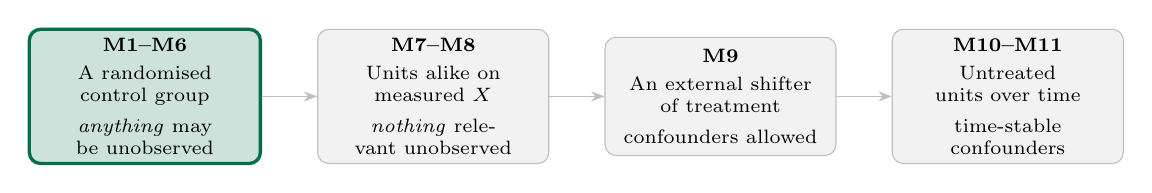
\begin{tikzpicture}[
    node distance=0.45cm and 0.7cm,
    box/.style={draw, rounded corners, minimum width=2.9cm, minimum height=1.5cm,
                font=\scriptsize, align=center, text width=2.7cm},
    active/.style={box, fill=sbgreen!20, draw=sbgreen, very thick},
    inactive/.style={box, fill=gray!10, draw=gray!50}
]
\node[active] (A) {\textbf{M1--M6}\\[2pt] A randomised control group\\[3pt] \emph{anything} may be unobserved};
\node[inactive, right=of A] (B) {\textbf{M7--M8}\\[2pt] Units alike on measured $X$\\[3pt] \emph{nothing} relevant unobserved};
\node[inactive, right=of B] (C) {\textbf{M9}\\[2pt] An external shifter of treatment\\[3pt] confounders allowed};
\node[inactive, right=of C] (D) {\textbf{M10--M11}\\[2pt] Untreated units over time\\[3pt] time-stable confounders};

\draw[-{Stealth}, gray!50] (A) -- (B);
\draw[-{Stealth}, gray!50] (B) -- (C);
\draw[-{Stealth}, gray!50] (C) -- (D);
\end{tikzpicture}
\end{center}

\bigskip

\begin{center}
\small The coin still supplies the counterfactual. What changes today is the question:\\
not \emph{does the coupon pay on average?} but \emph{for which customer does it pay?}
\end{center}
\end{frame}

% ====================================================================
\begin{frame}{Today's Plan}

\begin{center}
\small
\begin{tabular}{rp{11.6cm}}
\toprule
\textbf{Minutes} & \\
\midrule
0--15 & \textbf{Reading and critique C2} --- on paper, no devices \\
15--50 & \spinestep{Estimand:} two lists for 5{,}000 coupons; the CATE and the rule it feeds. \spinestep{Identification:} what the Q2 draw buys within every $x$ \\
60--110 & \spinestep{Estimation:} the interaction model and its predictions; is the gap noise?; S- and T-learners; fit, choose, assess \\
120--180 & \textbf{Lab 2:} structured outputs --- a language model codes a free-text field; check it against gold labels \\
\bottomrule
\end{tabular}
\end{center}

\bigskip

\textbf{Case:} Lin's coupon programme, Meeting 3 (Releases 1--5, and the Lab 2 opener). \quad \textbf{Released today:} the design menu; P2.

\bigskip

\textbf{Reading:} technical notes for Meeting 3. The earlier M3 workshop exercises are now Notebook 3.
\end{frame}

% ====================================================================
\begin{frame}{Critique C2: Five Questions, Every Time}

Read the one-page case silently. Notes on your own, then pairs, then the room.

\bigskip

\begin{enumerate}
    \item What is the claim?
    \item What causal question does the decision need?
    \item Who is the comparison group?
    \item What else could produce this pattern? Give the mechanism and the \textbf{direction} of the bias.
    \item What would you do to find out?
\end{enumerate}

\bigskip

\small C2's flaw is a Meeting 2 idea. Question 2 is where to find it: what threshold does the decision need? Hand in your notes at minute 15.
\end{frame}

% ====================================================================
\section{The Estimand: Whom to Coupon}
% ====================================================================

% [RELEASE R1 — the Q3 budget and the two proposed lists]
\begin{frame}{Two Lists for 5{,}000 Coupons}

M2 settled one question: \textbf{do not coupon everyone}. The CFO has approved \textbf{5{,}000 coupons} for Q3 --- half the base.

\bigskip
\pause

Two lists are on Lin's desk.

\begin{center}
\small
\begin{tabular}{p{5.4cm}p{6.8cm}}
\toprule
\textbf{Marketing's data science team} & \textbf{Lin} \\
\midrule
A purchase model on last year's transactions. Send to the 5{,}000 members most likely to buy. & Send to the 5{,}000 members the coupon \emph{moves} most. \\[0.4em]
\emph{``They are our best customers. They will redeem.''} & \emph{``That is exactly the problem.''} \\
\bottomrule
\end{tabular}
\end{center}

\bigskip
\pause

On the two segments of M1, marketing's model ranks the \textbf{active} members first (purchase rate $0.80$ with a coupon). Lin's rule ranks the \textbf{lapsed} first (lift $0.20$).
\end{frame}

% ====================================================================
\begin{frame}{The Number That Decides It}

From M1, per coupon sent to a customer with fields $x$:
\[
\text{net}(x) \;=\; \underbrace{30\,\tau(x)}_{\text{purchases caused}} \;-\; \underbrace{10\,\mu_1(x)}_{\text{coupons redeemed}},
\qquad \mu_1(x) = \E[Y(1) \mid X = x] .
\]

\pause

\begin{alertblock}{Coupon customer $x$ if and only if}
\[
\tau(x) \;>\; \frac{\mu_1(x)}{3}
\]
\end{alertblock}

\pause

\begin{center}
\small
\begin{tabular}{lrrrr}
\toprule
& $\tau(x)$ & $\mu_1(x)/3$ & \textbf{Net per coupon} & \textbf{5{,}000 coupons} \\
\midrule
Marketing's list (active) & 0.05 & 0.267 & \textcolor{warnred}{$-$\textyen 6.50} & \textcolor{warnred}{$-$\textyen 32{,}500} \\
Lin's list (lapsed) & 0.20 & 0.100 & \textcolor{sbgreen}{$+$\textyen 3.00} & \textcolor{sbgreen}{$+$\textyen 15{,}000} \\
\bottomrule
\end{tabular}
\end{center}

\medskip

The rule needs \textbf{two numbers per customer}. Every estimate today is a function of $x$; the question is which side of $\mu_1(x)/3$ it lands on, row by row.
\end{frame}

% [CARRIED VERBATIM from old-decks/lecture02.tex:726]
\begin{frame}{The CATE: Definition}

\begin{block}{Conditional Average Treatment Effect (CATE)}
\[
\tau(x) = \E[Y(1) - Y(0) \mid X = x] = \E[Y(1) \mid X = x] - \E[Y(0) \mid X = x]
\]
\end{block}

The CATE is a \textbf{function}, not a single number. The ATE is its average:

\[
\tau = \E[\tau(X)]
\]

\pause
\bigskip

\textbf{Identification under randomization:}
\[
\tau(x) = \E[Y \mid D = 1, X = x] - \E[Y \mid D = 0, X = x]
\]

This means: within each subgroup defined by $X = x$, the difference in means estimates the CATE.
\end{frame}

% [MOVED TO NOTES: CATE in Practice]

% [MOVED TO NOTES: A Taxonomy of Causal Estimands (Summary)]

% ====================================================================
\section{Identification: What Must Be True}
% ====================================================================

% [CARRIED VERBATIM from old-decks/lecture03.tex:154]
\begin{frame}{Identification of the CATE}
 
How do we go from potential outcomes ($\tau(x) = \E[Y(1) - Y(0) \mid X = x]$) to something we can estimate from data?
 
\bigskip
 
\begin{block}{Theorem (Identification of the CATE)}
Under (1) SUTVA, (2) independence: $D \indep (Y(1), Y(0)) \mid X$, and (3) overlap: $0 < \Prob(D = 1 \mid X = x) < 1$ for all $x$:
\[
\tau(x) = \E[Y \mid D = 1, X = x] \;-\; \E[Y \mid D = 0, X = x]
\]
\end{block}
 
\bigskip
 
\textbf{Proof.} By consistency: $\E[Y \mid D\!=\!1, X\!=\!x] = \E[Y(1) \mid D\!=\!1, X\!=\!x]$.
 
By independence: $\E[Y(1) \mid D\!=\!1, X\!=\!x] = \E[Y(1) \mid X\!=\!x]$.
 
Analogously for $D = 0$. Subtract. $\square$
 
\bigskip
 
This is the CATE analog of the ATE identification from M1.
\end{frame}

% [CARRIED VERBATIM from old-decks/lecture03.tex:181]
\begin{frame}{The Overlap Assumption}
 
Independence says treatment is ``as good as random'' given $X$.
 
\bigskip
 
\textbf{Overlap} says: for every type of customer $x$, there must be \emph{some} treated and \emph{some} control observations.
 
\[
0 < \Prob(D = 1 \mid X = x) < 1 \quad \text{for all } x
\]
 
\bigskip
 
Without overlap, the CATE is still well-defined, but may not be properly identified/estimated from the data.
 
\bigskip
 
\textbf{Example:} the chain runs an A/B test only among loyalty members. For non-members, $\Prob(D = 1 \mid X = \text{non-member}) = 0$. We never observe a treated non-member, so any estimate of $\mu_1(\text{non-member})$ is extrapolation, not a data-driven comparison.
\end{frame}

% Worksheet: pairs decide independence and overlap for each scenario before the answers frame.
% [CARRIED VERBATIM from old-decks/lecture03.tex:203]
\begin{frame}{Discussion: Do the Assumptions Hold?}
 
For each scenario, decide: does \textbf{independence} hold? Does \textbf{overlap} hold? What can we learn?
 
\bigskip
 
\begin{enumerate}
    \item \textbf{A/B test within loyal customers only}, random 50/50 within that group. Non-loyals are excluded.
 
    \medskip
 
    \item \textbf{Stratified A/B test:} gold-tier customers get the coupon with probability 70\%; silver-tier with probability 30\%. Assignment is random within each tier.
 
    \medskip
 
    \item \textbf{Coupons sent to customers who filed a complaint} in the past month; non-complainers get nothing.
 
    \medskip
 
    \item \textbf{Ride-hailing surge pricing} activated in high-demand zones; low-demand zones keep base price.
\end{enumerate}
 
\bigskip
\pause
 
\textcolor{gray}{\footnotesize Hint: for each, ask two questions. (a) Among the people you observe in treatment and control, is assignment independent of potential outcomes? (b) Are there subgroups where everyone (or no one) is treated?}
\end{frame}

% [REVISED from old-decks/lecture03.tex:232: independence vs overlap separated]
\begin{frame}{Discussion: Answers}

\begin{center}
\small
\begin{tabular}{p{3.2cm}p{2.2cm}p{1.9cm}p{4.6cm}}
\toprule
\textbf{Scenario} & \textbf{Indep.\ given $X$} & \textbf{Overlap} & \textbf{What can we learn?} \\
\midrule
A/B within loyals & \textcolor{sbgreen}{Yes} & \textcolor{warnred}{Loyals only} & $\tau(x)$ for loyals; non-loyal CATEs are extrapolation \\[0.5em]
Stratified 70/30 & \textcolor{sbgreen}{Yes} & \textcolor{sbgreen}{Yes} & $\tau(x)$ for all $x$; but $e(x) \neq 0.5$, so the pooled $\bar{Y}_1 - \bar{Y}_0$ is biased for the ATE \\[0.5em]
Coupons to complainers & trivially yes, given complaint & \textcolor{warnred}{No} & Nothing: no complainer is untreated, no non-complainer treated \\[0.5em]
Surge in high-demand zones & only if demand is recorded & \textcolor{warnred}{No} & Nothing from these data: price is a function of demand \\
\bottomrule
\end{tabular}
\end{center}

\bigskip

A \textbf{deterministic} rule makes independence given the rule's input automatic --- and useless, because overlap fails: there is no comparison left. Keep the two questions separate.
\end{frame}

% ====================================================================
\begin{frame}{What Must Be True, Sentence by Sentence}

From Lin's description of the Q2 export:

\bigskip

\begin{center}
\small
\begin{tabular}{p{6.4cm}p{6.6cm}}
\toprule
\textbf{The case says} & \textbf{Which buys} \\
\midrule
``The Q2 draw was 50/50 in every region, tier and store.'' & Independence \emph{within} every $x$, and $e(x) = 0.5$: overlap everywhere by design. \\[0.5em]
``All CRM fields were frozen the day before the draw.'' & $X$ is pre-treatment: no field can carry part of the effect. \\[0.5em]
``Members who joined during Q2 were not in the draw.'' & The CATE is identified only for pre-Q2 members. For new joiners it is extrapolation. \\
\bottomrule
\end{tabular}
\end{center}

\bigskip
\pause

The first two sentences make identification a fact about the procedure, as in M1. The third is about the \textbf{decision}: the Q3 list will include new members, and the test says nothing about them.

\medskip
\small The notebook's data-roles table from M1 gets one more column today: \emph{inside or outside the support}.
\end{frame}

% ====================================================================
\section{Estimation: The Interaction Model}
% ====================================================================

% [CARRIED VERBATIM from old-decks/lecture03.tex:255]
\begin{frame}{From Identification to Estimation}
 
Identification gives us:
\[
\tau(x) = \underbrace{\E[Y \mid D = 1, X = x]}_{\mu_1(x)} \;-\; \underbrace{\E[Y \mid D = 0, X = x]}_{\mu_0(x)}
\]
 
\bigskip
 
\textbf{Two functions to estimate.} How hard is this?
 
\bigskip
 
With two segments (active, lapsed): trivial. Compute within-group means.
 
\bigskip
 
With 10,000 customers and dozens of continuous features: we need a \textbf{model} for $\mu_1(x)$ and $\mu_0(x)$.
 
\bigskip
 
We start with the linear model, then generalize.
\end{frame}

% [CARRIED VERBATIM from old-decks/lecture03.tex:284]
\begin{frame}{Constant vs.\ Heterogeneous Effect}
 
\textbf{Constant effect model} (CUPED/ANCOVA from M2):
\[
Y_i = \alpha + \tau D_i + \beta X_i + \varepsilon_i \quad \Longrightarrow \quad \tau(x) = \tau \text{ for all } x
\]
$X$ is treated as purely prognostic: affects the \emph{level} but not the \emph{effect}.
 
\bigskip
\pause
 
\textbf{Heterogeneous effect model} (add an interaction):
\[
Y_i = \alpha + \tau D_i + \beta X_i + \gamma (D_i \times X_i) + \varepsilon_i
\]
 
\[
\Longrightarrow \quad \tau(x) = \tau + \gamma \, x
\]
 
\bigskip
 
$\gamma \neq 0$ means $X$ changes the treatment effect. $\beta$ captures the baseline difference across types.
\end{frame}

% ====================================================================
% [RELEASE R2 — four customers; pairs fill in the prediction columns before the \pause]
\begin{frame}{The Interaction Model: Both Worlds on Every Row}

$X = 1$ active, $X = 0$ lapsed. Solving from the four cell means of M1:
\[
\widehat\alpha = 0.10, \quad \widehat\tau = 0.20, \quad \widehat\beta = 0.65, \quad \widehat\gamma = -0.15
\]
\[
\widehat\mu_0(x) = \widehat\alpha + \widehat\beta x, \qquad \widehat\mu_1(x) = \widehat\alpha + \widehat\tau + (\widehat\beta + \widehat\gamma)x
\]

\pause

\begin{center}
\small
\begin{tabular}{lcccccc}
\toprule
\textbf{Customer} & $x$ & $D$ & $Y$ & $\widehat\mu_0(x)$ & $\widehat\mu_1(x)$ & \textbf{Coupon?} \\
\midrule
A & active & 1 & 1 & 0.75 & 0.80 & $0.05 < 0.267$: \textcolor{warnred}{no} \\
B & active & 0 & 1 & 0.75 & 0.80 & $0.05 < 0.267$: \textcolor{warnred}{no} \\
C & lapsed & 1 & 0 & 0.10 & 0.30 & $0.20 > 0.100$: \textcolor{sbgreen}{yes} \\
D & lapsed & 0 & 0 & 0.10 & 0.30 & $0.20 > 0.100$: \textcolor{sbgreen}{yes} \\
\bottomrule
\end{tabular}
\end{center}

\pause

\textbf{Aligned predictions:} both columns come from the \emph{same} row's $x$, whichever arm the row was in. $Y$ fills one column for each customer; the model fills both.

\smallskip
ATE check: $\widehat\tau + \widehat\gamma\,\E[X] = 0.20 - 0.15 \times 0.5 = 0.125$ $\checkmark$
\end{frame}

% ====================================================================
\begin{frame}{Read the Model Through Its Predictions}

\textbf{Coding sets the sign, not the substance.} With $X = 1$ active, $\tau(x) = 0.20 - 0.15x$. Recode $L = 1$ for lapsed: $\tau = 0.05 + 0.15L$. Same two effects.

\bigskip

\textbf{The coefficient on $D$ is not an average.} $\widehat\tau = 0.20$ is the effect at the reference group ($X = 0$, lapsed). To get the average for a population, \textbf{standardise with its weights}:

\begin{center}
\begin{tabular}{lrr}
\toprule
\textbf{Target population} & \textbf{Weights (active / lapsed)} & \textbf{Average effect} \\
\midrule
The whole base & 0.5 / 0.5 & $0.125$ \\
A list that is 80\% active & 0.8 / 0.2 & $0.8(0.05) + 0.2(0.20) = 0.08$ \\
\bottomrule
\end{tabular}
\end{center}

\bigskip

\textbf{A row's $\widehat\tau(x)$ is a group average.} A lapsed member's $0.20$ means about 200 extra purchases per 1{,}000 similar members --- not knowing \emph{which} 200.

\medskip

\small Standardisation is M2's transport again; it returns in M7 as identification from logs.
\end{frame}

% ====================================================================
\begin{frame}{From Two Segments to Fourteen Fields}

With two segments the CATE is two differences in means:
\begin{align*}
\tau(\text{active}) &= \E[Y \mid D\!=\!1, X\!=\!1] - \E[Y \mid D\!=\!0, X\!=\!1] = 0.80 - 0.75 = 0.05 \\
\tau(\text{lapsed}) &= \E[Y \mid D\!=\!1, X\!=\!0] - \E[Y \mid D\!=\!0, X\!=\!0] = 0.30 - 0.10 = 0.20
\end{align*}

Check: $\tau = 0.5 \times 0.05 + 0.5 \times 0.20 = 0.125$ $\checkmark$

\bigskip
\pause

\textbf{The Q2 export has 14 CRM fields} --- recency, visit frequency, tier, spend, app use, store, \ldots\ There are more cells than customers. We need models for
\[
\mu_1(x) = \E[Y \mid D = 1, X = x], \qquad \mu_0(x) = \E[Y \mid D = 0, X = x],
\]
then $\widehat\tau(x) = \widehat\mu_1(x) - \widehat\mu_0(x)$ --- and the decision uses $\widehat\mu_1(x)$ as well.

\bigskip

Any supervised learner can fit a $\mu$. The question is what goes wrong when it does.
\end{frame}

% ====================================================================
% [Case A: Part M3-R2b — the handout gives the counts; SEs on this frame after the attempt]
\begin{frame}{Is the Gap Itself Noise?}

Behind the segment rates: 200 members per arm in each segment of the Q2 test.

\begin{center}
\begin{tabular}{lrrrr}
\toprule
\textbf{Segment} & \textbf{Coupon} & \textbf{No coupon} & \textbf{Effect} & \textbf{SE} \\
\midrule
Active & 160/200 & 150/200 & $0.05$ & $\sqrt{\frac{0.16}{200} + \frac{0.1875}{200}} = 0.042$ \\
Lapsed & 60/200 & 20/200 & $0.20$ & $\sqrt{\frac{0.21}{200} + \frac{0.09}{200}} = 0.039$ \\
\bottomrule
\end{tabular}
\end{center}

\[
\widehat\tau_L - \widehat\tau_A = 0.15, \qquad \SE = \sqrt{0.042^2 + 0.039^2} = 0.057, \qquad z = 2.64 .
\]

\textbf{The heterogeneity is distinguishable from noise.} Test the \emph{gap}.

\bigskip

\begin{alertblock}{A common error}
``Significant for lapsed, not for active'' is not evidence of a difference. Active's $0.05$ has interval $[-0.03, 0.13]$: ``not significant'' is not ``zero''.
\end{alertblock}
\end{frame}

% ====================================================================
\section{Estimation: Handing the Job to ML}
% ====================================================================

% [MOVED TO NOTES: Limitations of the Linear Model]

% [CARRIED VERBATIM from old-decks/lecture03.tex:365]
\begin{frame}{S-Learner: The Natural First Attempt}
 
The interaction model is already a ``single model with $D$ as a feature.'' Just replace OLS with a flexible learner:
 
\bigskip
 
\textbf{Algorithm:}
\begin{enumerate}
    \item Include $D$ as a \textbf{feature} alongside $X$
    \item Fit a single model: $\hat{f}(x, d) \approx \E[Y \mid X = x, D = d]$
    \item $\hat{\tau}(x) = \hat{f}(x, 1) - \hat{f}(x, 0)$
\end{enumerate}
 
\bigskip
 
``S'' for ``single.'' Uses all $n$ observations.
 
\bigskip
 
Any base learner works: random forest, XGBoost, neural network, \ldots
 
\bigskip
 
This is the most direct generalization of what we just did with OLS.
\end{frame}

% [CARRIED VERBATIM from old-decks/lecture03.tex:392]
\begin{frame}{S-Learner: The Regularization Bias}
 
\begin{alertblock}{Problem}
$D$ is one feature among many. A regularized model (LASSO, random forest, XGBoost) may \textbf{shrink its effect toward zero}.
\end{alertblock}
 
\bigskip
 
The treatment signal competes with covariate signal for the model's ``attention.''
 
\bigskip
 
In the extreme: LASSO sets all interaction coefficients to zero $\Rightarrow$ $\hat{\tau}(x) = \hat{\tau}$ for all $x$. The model predicts $Y$ well (captures prognostic variation) but misses the heterogeneity entirely.
 
\bigskip
\pause
 
\textbf{Can we do better?} What if we avoid the competition between $D$ and $X$ entirely?
\end{frame}

% [CARRIED VERBATIM from old-decks/lecture03.tex:413]
\begin{frame}{T-Learner: Separate the Arms}
 
\textbf{Idea:} don't make $D$ compete with $X$. Instead, fit two completely separate models:
 
\begin{center}
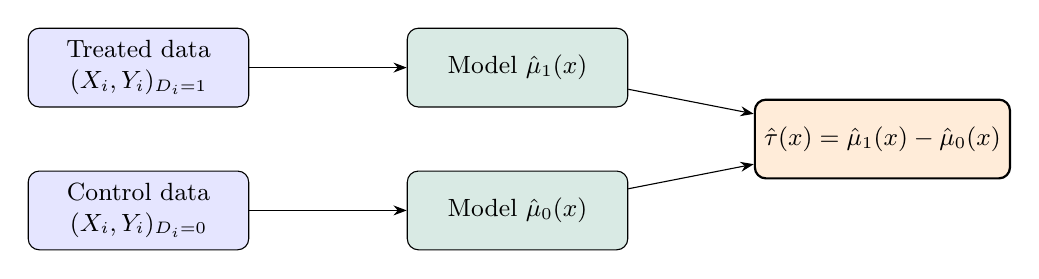
\begin{tikzpicture}[
    node distance=1.5cm and 2cm,
    box/.style={draw, rounded corners, minimum width=2.8cm, minimum height=1cm, font=\small, align=center},
    data/.style={box, fill=blue!10},
    model/.style={box, fill=sbgreen!15},
    result/.style={box, fill=orange!15, thick}
]
\node[data] (treat) {Treated data\\$(X_i, Y_i)_{D_i=1}$};
\node[data, below=0.8cm of treat] (ctrl) {Control data\\$(X_i, Y_i)_{D_i=0}$};
\node[model, right=of treat] (m1) {Model $\hat{\mu}_1(x)$};
\node[model, right=of ctrl] (m0) {Model $\hat{\mu}_0(x)$};
\node[result, right=3cm of $(m1)!0.5!(m0)$] (cate) {$\hat{\tau}(x) = \hat{\mu}_1(x) - \hat{\mu}_0(x)$};
 
\draw[-{Stealth}] (treat) -- (m1);
\draw[-{Stealth}] (ctrl) -- (m0);
\draw[-{Stealth}] (m1) -- (cate);
\draw[-{Stealth}] (m0) -- (cate);
\end{tikzpicture}
\end{center}
 
\bigskip
 
``T'' for ``two.'' Each model focuses on its own arm. No regularization can shrink the treatment effect, because $D$ never appears as a feature.
\end{frame}

% [CARRIED VERBATIM from old-decks/lecture03.tex:444]
\begin{frame}{T-Learner: The Variance Cost}
 
The T-learner solves the regularization bias. But it introduces a new problem:
 
\bigskip
 
\begin{alertblock}{Cost}
Each model sees only \textbf{half} the data. The two models are trained \textbf{independently}: no information sharing.
\end{alertblock}
 
\bigskip
 
If purchase history predicts outcomes similarly in both arms (prognostic variation), each model learns this pattern separately, wasting capacity.
 
\bigskip
 
Since the CATE is a \emph{difference}, the two fits' variances add, and their biases do not cancel unless they happen to be equal.
 
\bigskip
\pause
 
The S-learner shared \emph{too much}. The T-learner shares \emph{nothing}. Is there a middle ground?
\end{frame}

% ====================================================================
\begin{frame}{Better Fit, Worse Effect}

Lapsed members. Truth: $\mu_1 = 0.30$, $\mu_0 = 0.10$, so $\tau = 0.20$. Two fitted T-learners:

\begin{center}
\begin{tabular}{lrrrrr}
\toprule
& $\widehat\mu_1$ & $\widehat\mu_0$ & \textbf{Error in each} & $\widehat\tau$ & \textbf{Error in $\tau$} \\
\midrule
T-learner A & 0.34 & 0.14 & $+0.04$, $+0.04$ & 0.20 & \textcolor{sbgreen}{0} \\
T-learner B & 0.32 & 0.08 & $+0.02$, $-0.02$ & 0.24 & \textcolor{warnred}{$+0.04$} \\
\bottomrule
\end{tabular}
\end{center}

\bigskip

B fits \emph{both} outcomes better and gets the effect \emph{worse}. The effect's error is
\[
\widehat\tau - \tau = (\widehat\mu_1 - \mu_1) - (\widehat\mu_0 - \mu_0) :
\]
the difference of two errors. It cancels in A and compounds in B.

\medskip

\textbf{Outcome accuracy, arm by arm, does not grade an effect.} The next section shows the same thing at scale.
\end{frame}

% [CARRIED VERBATIM from old-decks/lecture03.tex:469]
\begin{frame}{Effect Modifiers vs.\ Prognostic Variables}
 
To understand the tradeoff, distinguish two kinds of covariates:
 
\bigskip
 
\textbf{Effect modifier:} a covariate $X_j$ such that $\tau(x)$ varies with $X_j$.
\begin{itemize}
    \item Segment at the coffee chain: $\tau(\text{lapsed}) = 0.20 \neq 0.05 = \tau(\text{active})$
    \item This is what we need for targeting
\end{itemize}
 
\bigskip
 
\textbf{Prognostic variable:} a covariate $X_j$ that predicts the outcome level $\E[Y \mid X]$ but does not change the treatment effect.
\begin{itemize}
    \item Commute distance: closer customers buy more, but the coupon effect is the same
    \item Helps with precision (CUPED, M2), not with targeting
\end{itemize}
 
\bigskip
 
The S-learner is good at prognostic variables but can miss effect modifiers. The T-learner detects effect modifiers but wastes capacity re-learning prognostic structure in each arm.
\end{frame}

% ====================================================================
\begin{frame}{Why This Bites at the Coffee Chain}

\textbf{Key fact:} most outcome variation is \emph{prognostic}.

\bigskip

On the two segments, the baseline gap between active and lapsed is $0.75 - 0.10 = 0.65$. The \emph{effect} gap is $0.20 - 0.05 = 0.15$. As variances across the base:
\[
\Var\bigl(\mu_0(X)\bigr) = 0.325^2 = 0.106, \qquad \Var\bigl(\tau(X)\bigr) = 0.075^2 = 0.0056 ,
\]
about \textbf{nineteen times} as much variation in \emph{who buys} as in \emph{who is moved}.

\pause
\bigskip

\begin{itemize}
    \item \textbf{S-learner} spends its capacity on the 0.65 gap. When $D$ explains a few percent of outcome variance, regularisation decides $D$'s interactions are not worth keeping.
    \medskip
    \item \textbf{T-learner} learns the 0.65 gap \emph{twice}, once per arm, each on half the data, and subtracts. Its errors in the big component land in the small one.
\end{itemize}

\bigskip

Both fit $Y$ well. Neither was asked to fit $\tau$.
\end{frame}

% [CARRIED VERBATIM from old-decks/lecture03.tex:590]
\begin{frame}{Summary: All Are Outcome Modeling}
 
\begin{center}
\begin{tabular}{p{2.5cm}p{4cm}p{4.5cm}}
\toprule
\textbf{Method} & \textbf{Strength} & \textbf{Weakness} \\
\midrule
\textbf{Linear model} & Simple, interpretable & Linearity; must specify interactions \\[0.6em]
\textbf{S-Learner} & All data; good at prognostics & Regularization shrinks effects \\[0.6em]
\textbf{T-Learner} & Flexible; detects effect modifiers & High variance; no sharing \\[0.6em]
\textbf{Multi-task} & Shares prognostic structure & More complex; needs large $n$ \\
\bottomrule
\end{tabular}
\end{center}
 
All four are \textbf{outcome modeling}: minimize prediction error for $Y$; the treatment effect falls out as a byproduct. None has a loss function that targets $\tau(x)$.  
 
\bigskip
 
An alternative: directly target $\tau(x)$. This is what causal trees and forests do (M4).
\end{frame}

% ====================================================================
\section{Estimation: Fit, Choose, Assess}
% ====================================================================

% [RELEASE R3 — the two-model comparison; pairs compute both RMSEs before the reveal]
\begin{frame}{Same RMSE, Opposite Decisions}

Two models of the two-segment world, fitted to 10{,}000 members split 50/50:

\begin{itemize}
    \item \textbf{Model I} (interaction): the four cell means exactly. $\widehat\tau(x) = 0.05$ or $0.20$.
    \item \textbf{Model A} (additive, no $D \times X$): $\widehat\mu = 0.1375 + 0.575x + 0.125D$. Every cell off by $\pm 0.0375$; $\widehat\tau(x) = 0.125$ for everyone.
\end{itemize}

\pause

\begin{center}
\small
\begin{tabular}{lrrr}
\toprule
& \textbf{Outcome RMSE} & $\widehat\tau(x)$ & \textbf{5{,}000 coupons ranked by $\widehat\tau$} \\
\midrule
Model I & $\sqrt{0.16188} = 0.4023$ & 0.05 / 0.20 & lapsed first: \textcolor{sbgreen}{$+$\textyen 15{,}000} \\
Model A & $\sqrt{0.16188 + 0.0375^2} = 0.4041$ & 0.125 / 0.125 & a coin toss: \textcolor{warnred}{$-$\textyen 8{,}750} \\
\bottomrule
\end{tabular}
\end{center}

\smallskip
\small $0.16188$ is the irreducible part: the average of $p(1-p)$ over the four cells. Random ranking: $5{,}000 \times \tfrac12(-6.50 + 3.00)$.

\pause
\medskip
\normalsize

The RMSEs differ by \textbf{0.4\%}. The decisions differ by \textbf{\textyen 23{,}750}. A purchase has a coin-flip's worth of noise in it; the heterogeneity that pays is a rounding error to an outcome loss.
\end{frame}

% ====================================================================
% [RELEASE R4 — the full Q2 export; predictions go on the board]
\begin{frame}{The Q2 Export}

\begin{center}
\small
\begin{tabular}{lr}
\toprule
Members in the Q2 draw, all three test regions & \NUM{10{,}000}{sim coupon-q2 v2: members in the export} \\
CRM fields, frozen before the draw & 14 \\
Coupon arm / control arm & 50\% / 50\% \\
Coupons available for the Q3 list & 5{,}000 \\
\bottomrule
\end{tabular}
\end{center}

\bigskip
\pause

Four learners, each fitted on the same training folds:

\begin{center}
\small
(1) interaction OLS: $D$, 14 fields, $D \times$ each field \quad (2) S-learner, lasso\\
(3) S-learner, boosted trees \quad (4) T-learner, boosted trees
\end{center}

\bigskip

\textbf{In pairs, predict:} which has the best out-of-fold outcome RMSE? Which list of 5{,}000 earns the most? Are they the same learner?

\begin{center}\small Commit before the next slide.\end{center}
\end{frame}

% ====================================================================
% [RELEASE R5 — the ladder; the simulation's truth is shown only here]
\begin{frame}{The Ladder}

\begin{center}
\scriptsize
\begin{tabular}{lrr}
\toprule
\textbf{Learner} & \textbf{Outcome RMSE} & \textbf{Net, 5{,}000 coupons (\textyen)} \\
\midrule
Interaction OLS & \NUM{0.412}{sim v2: OOF RMSE, interaction OLS} & \NUM{$+$4{,}100}{sim v2: true net, top-5000 by tau-hat, interaction OLS} \\
S-learner, lasso & \NUM{0.409}{sim v2: OOF RMSE, S-lasso} & \NUM{$-$6{,}800}{sim v2: true net, S-lasso list} \\
S-learner, boosted & \textbf{\NUM{0.401}{sim v2: OOF RMSE, S-boosted}} & \NUM{$+$1{,}900}{sim v2: true net, S-boosted list} \\
T-learner, boosted & \NUM{0.406}{sim v2: OOF RMSE, T-boosted} & \textbf{\NUM{$+$9{,}300}{sim v2: true net, T-boosted list}} \\
\midrule
\textit{List by the true $\tau(x)$} & --- & \textcolor{sbgreen}{\NUM{$+$16{,}200}{sim v2: true net, oracle list}} \\
\textit{Marketing's purchase model} & --- & \textcolor{warnred}{\NUM{$-$29{,}400}{sim v2: true net, top-5000 by predicted purchase}} \\
\bottomrule
\end{tabular}
\end{center}

\end{frame}

% ====================================================================
\begin{frame}[shrink=6]{Fit, Choose, Assess}

The best RMSE and the best list came from \textbf{different} learners, and every learner beat marketing's list: the \emph{question} was the bigger error. So how should one choose? Every row gets one of three roles:

\begin{center}
\small
\begin{tabular}{llp{6.4cm}}
\toprule
\textbf{Role} & \textbf{Rows} & \textbf{What happens there} \\
\midrule
Fit & training folds & Each learner estimates $\widehat\mu_1, \widehat\mu_0$ \\
Choose & validation fold & Pick one learner. \textcolor{warnred}{Not by outcome RMSE:} it is blind to $\tau$ \\
Assess & held-out test & Touched once: the value of the chosen list \\
\bottomrule
\end{tabular}
\end{center}

\pause
\medskip

The difficulty is the middle row. $\tau_i$ is never observed, so ``RMSE of $\widehat\tau$'' cannot be computed on real data. Outcome RMSE can, and it measures the wrong thing: its gap from ignoring all heterogeneity is only $\Var(\tau(X))/4$ (notes).

\medskip

\textbf{What can be computed} on a randomised validation fold is the \emph{value of the list} a learner produces --- the lift among the customers it picks. That is M5.

\medskip
\small Split \textbf{members} into folds before creating any per-visit or duplicated rows, or the same member leaks across roles. Today the simulation lets us cheat and see the truth. Your data will not.
\end{frame}

% ====================================================================
\begin{frame}{Key Takeaways}

\begin{itemize}
    \item \spinestep{Estimand.} Targeting needs $\tau(x)$, not $\Prob(\text{buy} \mid x)$: coupon $x$ iff $\tau(x) > \mu_1(x)/3$. A list's average effect uses \emph{that list's} weights.
    \item \spinestep{Identification.} The Q2 draw identifies $\tau(x)$ within every $x$ --- only on the test's support. New members are extrapolation. Deterministic rules fail on overlap.
    \item \spinestep{Estimation.} Every learner here is outcome modelling: predict both potential outcomes on the same row, subtract. Test the \emph{gap} between segments, not two significance labels.
    \item \textbf{S-learners shrink the effect; T-learners learn the baseline twice.} Both fail for the same reason: prognostic variation dwarfs the effect. A better fit to each arm can give a worse effect.
    \item \textbf{Choose by the decision, not by the fit.} Outcome RMSE barely sees heterogeneity worth \textyen 23{,}750.
\end{itemize}

\medskip

\small \textbf{Due 48 hours from now:} your pair's question and data idea, one page. Use the design menu. \quad \textbf{P2} (causal audit skill) is released tonight.
\end{frame}

% ====================================================================
\begin{frame}[shrink=2]{Lab 2: A Column Written by a Language Model}

Case A, Lab 2 opener: a model reads members' app feedback and labels them ``drifting away: yes/no''. Sixty minutes.

\medskip

\begin{center}
\scriptsize
\begin{tabular}{rlp{8.6cm}}
\toprule
\textbf{Min} & \textbf{Slot} & \textbf{Task} \\
\midrule
5  & Task and schema & Write the output schema: one typed field, allowed values, and a ``cannot tell'' option. Only comments written \emph{before} the Q2 draw may be coded. \\
10 & Demonstration & Structured output against the schema through the course wrapper; a prompt that violates the schema and one that does not. \\
30 & Build & Code the pre-draw comments. Measure accuracy against the 200 gold labels, separately for lapsed and active members. \\
10 & Verify & Re-estimate the segment effects using the coded label. Compare with the CRM flag: how far did the gap shrink, and what does the coded list earn? \\
5  & Interpret & One sentence: at your measured accuracy, would you target on the coded field? (Break-even accuracy, by hand: $0.684$.) \\
\bottomrule
\end{tabular}
\end{center}

\small \textbf{Close:} a model-coded covariate is a measurement with error. Misclassification pulls segment effects toward each other, and it is invisible unless you check against gold labels. The earlier M3 workshop (aligned predictions, penalty sweep, RMSE vs value) is Notebook 3.
\end{frame}

\end{document}
